\documentclass[12pt]{article}

\usepackage{sbc-template}
\usepackage{graphicx,url}
\usepackage[utf8]{inputenc}
\usepackage[brazil]{babel}

\usepackage{listings}
\usepackage{xcolor}
\usepackage{colortbl}
\usepackage{graphicx}
\usepackage{amsmath}
\usepackage{centernot}

\colorlet{punct}{red!60!black}
\definecolor{background}{HTML}{EEEEEE}
\definecolor{delim}{RGB}{20,105,176}
\colorlet{numb}{magenta!60!black}

\lstdefinelanguage{json}{
    basicstyle=\normalfont\ttfamily,
    numbers=left,
    numberstyle=\scriptsize,
    stepnumber=1,
    numbersep=8pt,
    showstringspaces=false,
    breaklines=true,
    frame=lines,
    backgroundcolor=\color{background},
    literate=
     *{0}{{{\color{numb}0}}}{1}
      {1}{{{\color{numb}1}}}{1}
      {2}{{{\color{numb}2}}}{1}
      {3}{{{\color{numb}3}}}{1}
      {4}{{{\color{numb}4}}}{1}
      {5}{{{\color{numb}5}}}{1}
      {6}{{{\color{numb}6}}}{1}
      {7}{{{\color{numb}7}}}{1}
      {8}{{{\color{numb}8}}}{1}
      {9}{{{\color{numb}9}}}{1}
      {:}{{{\color{punct}{:}}}}{1}
      {,}{{{\color{punct}{,}}}}{1}
      {\{}{{{\color{delim}{\{}}}}{1}
      {\}}{{{\color{delim}{\}}}}}{1}
      {[}{{{\color{delim}{[}}}}{1}
      {]}{{{\color{delim}{]}}}}{1},
}

     
\sloppy

\title{Placidus: Uma Plataforma de Verificação Formal para Redes Definidas por Software}

\author{Levindo Gabriel Taschetto Neto\inst{1}, Alberto Egon Schaeffer-Filho\inst{1}}


\address{Instituto de Informática -- Universidade Federal do Rio Grande do Sul
  (UFRGS)\\
  Caixa Postal 15.064 -- 91.501-970 -- Porto Alegre -- RS -- Brazil
  \email{\{lgtneto,alberto\}@inf.ufrgs.br}
}

\begin{document} 

\maketitle

\begin{abstract} %#meia pagina
Formal verification is an important step in checking network operations and ensuring properties, for instance, the accuracy of device configurations. Nevertheless, historically, formal verification techniques are limited by performance, scalability, and expressiveness, mainly due to the complexity of the current networks.
Problems on processing a specificic task or function in computer networks may be critical for the reliability of a whole system.
In order to solve these possible complications, several techniques for formal verification can be used, such as (i) updating the information about the context and state of network devices, and (ii) using intelligent strategies for combining representation models for guaranteeing performance and scalability.
Software defined networking (SDN) architectures offer the essence needed for resolving this kind of issue.
It enables the selection of a set of different techniques for increasing the quality of the results obtained by a selection system.
In this paper, we propose the Placidus framework, which is a platform for formal verification in software defined networking.
The framework is flexible and capable of verifying a large range of network properties, such as reachability, redundancy in network devices, and other inconsistencies.
\end{abstract}
     
\begin{resumo}  %#meia pagina
Verificação formal é um passo importante na checagem de operações e propriedades em redes de computadores, como por exemplo, a corretude das configurações de dispositivos inseridos na mesma. Entretanto, historicamente, técnicas de versão formal são limitadas por performance, escalabilidade e expressividade, principalmente devido à complexidade das redes de computadores atuais.
Problemas para processar uma tarefa ou função específica em uma rede podem ser críticos para a confiabilidade de um sistema como um todo.
Para resolver essas complicações possíveis, várias técnicas para verificação formal podem ser utilizadas, tais como (i) atualização das informações sobre os contextos e estados de dispositivos da rede e (ii) utilização de estratégicas inteligentes para combinar modelos de representação para garantir performance e escalabilidade.
Arquiteturas para Redes Definidas por Software (\textit{SDN}) oferecem a essência necessária para resolver problemas desse tipo, uma vez que disponibilizam a combinação de diferentes técnicas para aumentar a qualidade dos resultados obtidos por um sistema de seleção.
Nesse trabalho, nós propomos o framework Placidus, que é uma plataforma para verificação formal em \textit{SDN}.
O framework é flexível e capaz de verificar um grande número de propriedades, como alcançabilidade, redundância, conflitos, entre outras inconsistências em dispositivos de rede.

\end{resumo}


\section{Introdução}  %#1 pagina

De acordo com \cite{Feamster_2005}, protocolos legados, tais como \textit{BGP (Border Gateway Protocol)} \cite{569372}, ainda sofrem com problemas de configuração, principalmente devido a enganos causados por operadores de rede.
Essa realidade expõe a necessidade de estudos voltados à detecção desse tipo de erro e a classificação de sua origem como maliciosa ou ocasional. Estudos tais como \cite{6679403} sugerem que verificação formal possui um conjunto de técnicas capaz de verificar ambientes de rede e responder essas questões, já que é uma área ampla, incluindo técnicas tais como \textit{model checking}\footnote{Procedimento de verificação formal para saber se um modelo cumpre uma especificação dada por uma propriedade expressada formalmente em termos de uma fórmula lógica temporal.} e \textit{symbolic simulation}\footnote{Forma de simulação onde diversas execuções possíveis de um sistema são consideradas simultaneamente.} para o tratamento de diversos tipos de inconsistências mesmo em diferentes domínios. Existe uma necessidade adicional de que técnicas de verificação formal sejam sofisticadas, utilizando o contexto e estado dos dispositivos de rede, modelos de representação precisos e estratégias de remediação.

Apesar de o uso de técnicas de verificação formal de forma isolada ser frequente conforme evidenciado por trabalhos como \cite{Ball_2014}, nós entendemos que a combinação de técnicas de verificação distintas mas complementares é importante.
Afinal, o uso dessas (i) permite a elaboração de estratégias complexas onde uma técnica serve de entrada para outra criando uma cadeia de verificação capaz de aumentar a acurácia global do sistema; (ii) permite a atualização de técnicas conforme a necessidade da rede, uma vez que pode haver atualização de uma regra específica enquanto outra não é mudada, mantendo a rede estável; (iii) permite tratar uma gama maior de erros na rede visto que técnicas que abordam domínios complementares podem ser utilizadas juntas.

Arquiteturas \textit{SDN} oferecem o ferramental necessário para aplicação de métodos formais para verificação de protocolos e aplicações de rede \cite{6873212}.
Contudo, ainda existem desafios como (i) detectar falha de configuração proveniente da interação humana nesses ambientes, (ii) auxiliar a rede a inserir e remover aplicações sem desconfigurar seus dispositivos e (iii) coordenar a interação conjunta de aplicações distintas e complexas de modo que uma não interfira no funcionamento da outra. Mesmo que as funcionalidades da programação e do controle centralizado que \textit{SDN} oferecem simplifiquem drasticamente o gerenciamento da rede e permitam inovações na mesma, ainda é um ambiente com grandes necessidades de verificação, já que a sua programabilidade aumenta o risco de erros na rede \cite{8691107}.

A estrutura desse trabalho é como segue: a Seção 2 apresenta conceitos básicos e técnicos referentes: (i) à verificação formal, (ii) a protocolo OpenFlow e (iii) a redes definidas por software.
A Seção 3 apresenta a arquitetura do \textit{framework} proposto e o plano de avaliação para a solução desenvolvida.
A Seção 4, por fim, apresenta o cronograma de atividades que será utilizado como base para a segunda etapa desse trabalho.

\section{Fundamentação Teórica}

Nesta seção apresentamos uma fundamentação teórica no contexto do qual o framework Placidus está inserido. Em particular, discutimos sobre verificação formal, protocolo OpenFlow, redes definidas por software, estado da arte na área em que a solução está inserida e trabalhos relacionados ao framework proposto.

\subsection{Verificação Formal}

Verificação formal engloba um conjunto de técnicas, tais como \textit{model checking} \cite{8914133}, para validação baseada em lógica matemática para demonstrar formalmente que um software, ou um hardware, implementa de maneira correta as funcionalidades que foram estabelecidas no projeto.
Técnicas de Verificação formal têm sido muito importantes em processos de validação, como por exemplo na fabricação de circuitos integrados \cite{8894278}.

Em geral, é utilizada para verificar configurações de rede fixa, como o comportamento de encaminhamento de um determinado pacote. Geralmente, inclui técnicas como verificação de modelos \cite{655848}, simulação simbólica \cite{7127376} e reduções \textit{SAT} \cite{5958483}. Historicamente, a verificação de modelo aplicada à verificação estática usa \textit{snapshots} de rede para obter uma visão global da atividade da mesma. Outra técnica frequentemente utilizada é a simulação simbólica \cite{7059250}. 
Como desvantagem, muitas vezes a interferência manual é necessária para adicionar axiomas\footnote{Expressões universalmente válidas e verdadeiras.} que o sistema não pode considerar automaticamente~ \cite{ModelCheckerSDN}.

\subsection{Verificação Estática}

No contexto de redes definidas por software, é o conjunto de processos para análise de determinada topologia de rede. 
Esse conjunto serve para identificar e testar regras formadas por fluxos de rede que estão circulando, na mesma, no instante da verificação \cite{8536203}.
Para capturar as informações dos dados, que estão trafegando na rede em determinado instante, faz-se a utilização de \textit{snapshots} \cite{8855530}.

Os \textit{snapshots} são registros instantâneos de fluxos que estão presentes, em determinado momento, em um plano de dados \textit{SDN}.
Eles também são utilizados em outras áreas, como em sistemas distribuídos \cite{7903947}, com a função de monitoramento.
A partir da captura dos \textit{snapshots}, é possível fazer a verificação das regras contidas nos mesmos.
As regras se apresentam na forma lógica, e podem ser validadas com o uso de verificação formal estática.

\subsection{Protocolo OpenFlow}
Diversas aplicações de rede podem utilizar as informações oferecidas pelo controlador para construir funções de alto nível sobre a rede física, como por exemplo, virtualização ou controle de tráfego  \cite{6936857}. 
Em 2008, um grande impulso foi dado a essa ideia geral, culminando no protocolo OpenFlow \cite{Mckeown_2008}, o qual é um padrão de redes definidas por software. Proposto por Nick Mckeown, a especificação do protocolo foi muito bem aceita pela academia e indústria devido a, principalmente, sua facilidade de implantação.

De fato, todas as funcionalidade propostas na primeira versão do protocolo já existiam nos dispositivos da época ou podiam ser alcançadas com uma simples atualização de \textit{firmware} \cite{Feamster_2010}.
Desse modo, a indústria não representou uma limitação para essa nova investida. Ademais, representa uma plataforma para inovação em \textit{SDN}.

\subsubsection{Tabelas de Fluxo}
A tabela de fluxo no protocolo OpenFlow consiste de entradas de regras, representadas pelos componentes: (i) \textit{match}, (ii) prioridade, (iii) contadores, (iv) instruções, (v) \textit{timeouts} e (vi) cookie \cite{654135}.
Os campos de \textit{match} contêm a porta de ingresso no switch e os cabeçalhos de pacotes, além de opcionalmente possuírem metadados referentes a uma tabela associada.
Já o campo de prioridade conta com a precedência de casamento de regras de entrada de fluxo.

Os contadores são os campos que possuem seu valor incrementado quando os pacotes têm regras casadas entre si. Já o campo de instruções é utilizado para fazer modificações no conjunto de ações de determinada regra. O campo referente aos \textit{timeouts} possui o tempo de expiração do fluxo dentro do switch\footnote{Equipamento ativo que funciona normalmente na camada de enlace do Modelo OSI e tem como principal funcionalidade a interligação de equipamentos de uma rede.}. O campo de cookie, por sua vez, contem valores de dados opacos\footnote{Tipos de dados os quais suas estruturas de dados não são definidas por uma interface.} escolhidos pelo controlador, e deve ser utilizado pelo mesmo para filtrar estatísticas, modificações e deleções dos fluxos contidos na rede.

\subsubsection{Tipos de Mensagens}
As mensagens do protocolo OpenFlow são divididas em duas categorias: (i) assíncronas e (ii) simétricas. Dentre as mensagens assíncronas têm-se (i) \textit{oftp\_packet\_in}, para pacotes recebidos e mandados ao controlador; (ii) \textit{oftp\_flow\_removed}, para notificar o controlador se um fluxo atinge seu tempo de expiração ou se é removido da tabela de fluxos; (iii) \textit{oftp\_port\_status}, para notificar o controlador sobre alterações em portas, além de remoções e adições das mesmas; e (iv) \textit{oftp\_error\_msg}, para notificar o controlador sobre algum problema no switch OpenFlow.

As mensagens simétricas, por outro lado, são constituídas por (i) \textit{oftp\_hello}, que consiste de um cabeçalho OpenFlow mais um conjunto de elementos \textit{hello} de tamanho variável; (ii) \textit{echo request}, a qual consiste de um cabeçalho OpenFlow juntamente a um campo de dados de tamanho arbitrário; (iii) \textit{echo reply}, que consiste também em um cabeçalho OpenFlow, mas com um campo de dados não modificado de uma mensagem de \textit{echo request}; e (iv) \textit{experimenter}, o qual possui o mesmo cabeçalho das demais mensagens, mas com um campo \textit{experimenter} de 32 bits para identificação e um campo de tipo, também sendo um inteiro sem sinal de 32 bits \cite{654135}.

\subsubsection{Canal Seguro}

O canal seguro do protocolo OpenFlow é o caminho usado para comunicações entre o controlador OpenFlow o dispositivo OpenFlow.
Geralmente, essa comunicação tem segurança fornecida por encriptação assimétrica baseada em TLS (\textit{Transport Layer Security}).
No entanto, conexões TCP\footnote{O Protocolo de Controle de Transmissão é um padrão que define como estabelecer e manter uma conversação de rede para que aplicações possam transferir dados entre si.} sem encriptação são permitidas \cite{Goransson:2014:SDN:2671152}.

Essas conexões podem ser \textit{in-band}\footnote{Esse tipo de conexão usa os mesmos enlaces (i.e., mesma rede) para ambos tráfego de controle e de dados.} ou \textit{out-of-band}\footnote{Esse tipo de conexão usa portas e enlaces Ethernet separados (i.e., rede separada) para conectar dispositivos de encaminhamento ao controlador.}.
Algumas arquiteturas legadas de rede ainda entregam mensagens OpenFlow via canal seguro para o mesmo ter todo o processamento (tratamento e parseamento) dentro do switch.
Dessa forma, o canal seguro \textit{out-band} é relevante apenas no caso de um switch OpenFlow híbrido.

\subsection{Redes Definidas por Software (\textit{SDN})}

Tradicionalmente, a lógica de encaminhamento de pacotes se encontra embutida nos equipamentos responsáveis por essa função, e essa arquitetura é a que encontramos na maior parte da Internet atualmente.
Essa forma de arquitetura de rede permitiu grandes avanços quanto à autonomia dos dispositivos. Não obstante, essa enrijeceu e desacelerou a inovação de protocolos e funções de rede inserindo uma complexidade alta na implantação e teste de novas ideias  \cite{Mckeown_2008}.

\textit{SDN} tem como propósito fundamental o desacoplamento do plano de controle do plano de dados via protocolo OpenFlow, dentro da camada de rede do Modelo OSI \cite{1094702}.
O plano de controle em redes definidas por software é concentrado em um controlador logicamente centralizado e uma aplicação em seu topo \cite{2228312}.
Já o plano de dados é um \textit{snapshot} da tabela de encaminhamento dos dispositivos de rede.
A diferença entre esses dois planos pode ser observada na Tabela \ref{table:pdpc}.

Entre outras atividades, fica a cargo do controlador definir como o roteamento de dados será feito na rede. Os dispositivos responsáveis pelo encaminhamento de dados são denominados genericamente de switches e residem na porção da arquitetura de rede chamada plano de dados. Assim, há uma grande separação entre as funções oferecidas pelo plano de controle e plano de dados. Essa separação oferece uma maior modularização e flexibilidade quanto ao software utilizado, inserindo uma alta camada de abstração sobre os recursos de rede, e fornecendo meios para alcançar o conceito de maior programabilidade de rede.
Desse modo, \textit{SDN} representa uma plataforma para inovação com inúmeras possibilidades e desafios. 

\begin{table}[]
\resizebox{\textwidth}{!}{
    \begin{tabular}{|l|l|l|ll}
        \cline{1-3}
        & \begin{tabular}[c]{@{}l@{}}Plano de Dados\end{tabular} & \begin{tabular}[c]{@{}l@{}}Plano Controle\end{tabular} &  &  \\ \cline{1-3}
        Definição & \begin{tabular}[c]{@{}l@{}}Coleção de tabelas de encaminhamento\\ e lógicas de encaminhamento de pacotes\end{tabular} & \begin{tabular}[c]{@{}l@{}}Programa constrói as tabelas de\\ encaminhamento com topologia e enlaces\end{tabular} &  &  \\ \cline{1-3}
        Propriedades de objeto imutáveis para todos pacotes & Ficam junto às tabelas de encaminhamento & Ficam junto às configurações da topologia &  &  \\ \cline{1-3}
        Tipos de Programas & Tabela de fluxos em \textit{SDN} & BGP, OSPF \cite{8863947}, etc &  &  \\ \cline{1-3}
    \end{tabular}
}
\caption{Plano de Dados vs Plano de Controle. Fonte: obtido pelo autor, 2019.}
\label{table:pdpc}
\end{table}

\subsection{Estado da Arte em Verificação Formal em Redes Definidas por Software} 

Muitos estudos têm se concentrado no contexto de verificação de dispositivos de redes definidas por software.
O \textit{framework} proposto nesse trabalho, o Placidus, faz a verificação, de maneira formal, de dispositivos em \textit{SDN} no plano de controle da camada de rede do Modelo OSI \cite{1094702}.

Todavia, estudos nessa área têm sido desenvolvidos para a o plano de dados da mesma camada.
Muitas universidades e empresas, incluindo as de grande porte como Microsoft e Stanford, criaram grupos de pesquisa focados em verificação de redes de computadores \cite{123456}.

\subsection{Trabalhos Relacionados}

O advento do protocolo OpenFlow facilitou o teste de soluções no ambiente de redes definidas por software.
Sendo assim, pesquisas bastante relevantes estão relacionados ao \textit{framework} proposto nesse trabalho no que tange as propriedades verificadas.
Entre eles, O \textit{PreChecker} \cite{8738806}, o qual encontra dinamicamente conflitos e computa pacotes de classes equivalentes para verificações dentro do plano de controle. O mesmo faz uso de uma estrutura \textit{MTBDD} (Diagramas Multi-Terminais de Decisão Binária) para representar a agregação de regras dominantes.

Para verificação de regras redundantes e conflitantes, um trabalho com bastante relevância é o \textit{SUPC (SDN enabled Universal Policy Checking)} \cite{8685550}, que é uma composição de funções de serviços (\textit{SFs}) automatizado e um framework para análise de conflitos e redundâncias.
O \textit{SUPC} traduz tráfego e políticas de segurança de vários \textit{SFs} para um formato OpenFlow comum, o que auxilia na eliminação de regras redundantes.

Outro trabalho bastante relevante nessa área é o \textit{CDD (Covert
Channel Defender)} \cite{8428482}, que objetiva a resolução de conflitos entre regras no plano de dados da camada de rede.
O \textit{CDD} rastrea cada evento modificação de regra, e executa algoritmos eficientes para resolver conflitos entre regras, em tempo real.
Ademais, assim como o Placidus, o \textit{CDD} utiliza o controlador \textit{opensource} Floodlight \cite{7491821} e teve seus testes executados numa rede emulada com o emulador de rede Mininet \cite{6860404}.

Em propriedades tais como \textit{reachability}, um trabalho que se destaca é o \cite{8342927}, o qual usa um método de detecção baseado em modelo de caminhamento em árvore, o qual pode rapidamente detectar regras na rede e prover conveniência a administradores que gerenciam as mesmas. Esse método reduz a complexidade de autenticação na rede como um todo por estabelecimento da topologia com cada porta dos switches. Além disso, A decisão de alcançabilidade entre dois vértices pode ser avaliada num tempo constante através de um conjunto de operações preestabelecido.


\section{O Placidus}

O framework Placidus conta com uma arquitetura modular, e se encontra acima do plano de controle da rede, utilizando dados providos pelo controlador Floodlight\footnote{http://www.projectfloodlight.org/floodlight}.
Além disso, faz uso de uma rede emulada pelo emulador Mininet\footnote{http://mininet.org}.

O Placidus está subdividido em três grandes módulos: (i) coleta de dados, (ii) verificador de conflitos e redundâncias e o (iii) verificador de \textit{reachability}. Outras propriedades estão sendo avaliadas para serem implementadas (e.g.: \textit{slice isolation} e \textit{black hole}) como novos módulos da plataforma.
Ademais, uma integração com um banco de dados para coleta e armazenamento dos dados obtidos será implementada, sendo mais uma funcionalidade do Placidus, assim como a infraestrutura para rodar a plataforma.

\subsection{Visão Geral do Framework}

O Placidus faz o uso de diferentes técnicas algorítmicas para executar suas verificações.
Os predicados contêm predicados atômicos, onde cada um representa uma especificação de ação a ser tomada por um pacote quando esse chega em determinado dispositivo da topologia.
No módulo de verificação de conflitos e redundâncias, cada regra é formada por um produtório de predicados atômicos implicando em uma ação.
Nesse módulo, é utilizado um algoritmo de comparação entre regras, o qual faz a checagem de dois em dois fluxos para saber se há conflito ou redundância, mas sempre removendo o primeiro fluxo da lista provida pela \textit{flow table}.

Já no módulo de verificação de \textit{reachability}, técnicas com o uso de vetores de bits são utilizadas. Cada fluxo dentro da topologia de rede, que é modelada na forma de um grafo\footnote{Estrutura de dados que representa valores conectados em um espaço multidimensional.}, é convertido para um conjunto de bits ordenados, onde os bits menos significativos representam o \textit{match}, e os mais significativos a ação do fluxo.
As verificações entre fluxos podem ser feitas então por operadores lógicos (e.g.: \textit{XNOR} e \textit{AND}).
Os dados utilizados para essas verificações podem ser obtidos de maneira simples pelo menu inicial do Placidus. Esse menu também conta com as opções para (i) gerar/atualizar a tabela de dados de verificação, (ii) adicionar mais regras ao controlador, (iii) deletar regras do controlador e (iv) ver todas regras contidas no controlador de rede.

\subsection{Arquitetura do Placidus}
O módulo de coleta de dados se comunica com os outros dois módulos, uma vez que ele participa do início de todas verificações de propriedades realizadas pelo \textit{framework} apresentado nesse trabalho.
Os módulos de verificação não se comunicam entre si, já que ambos possuem suas próprias funções e estruturas de dados.
Essa não comunicação entre os módulos de verificação faz com que o Placidus possua um baixo acoplamento e uma alta coesão entre seus blocos de verificação, o que faz com que a arquitetura do mesmo seja mais organizada e flexível \cite{5229862}.
A arquitetura inicial proposta para o framework pode ser observada na Figura \ref{fig:ArquiteturaPlacidus}.

 \begin{figure}[!ht]
     \centering
     \fbox{
         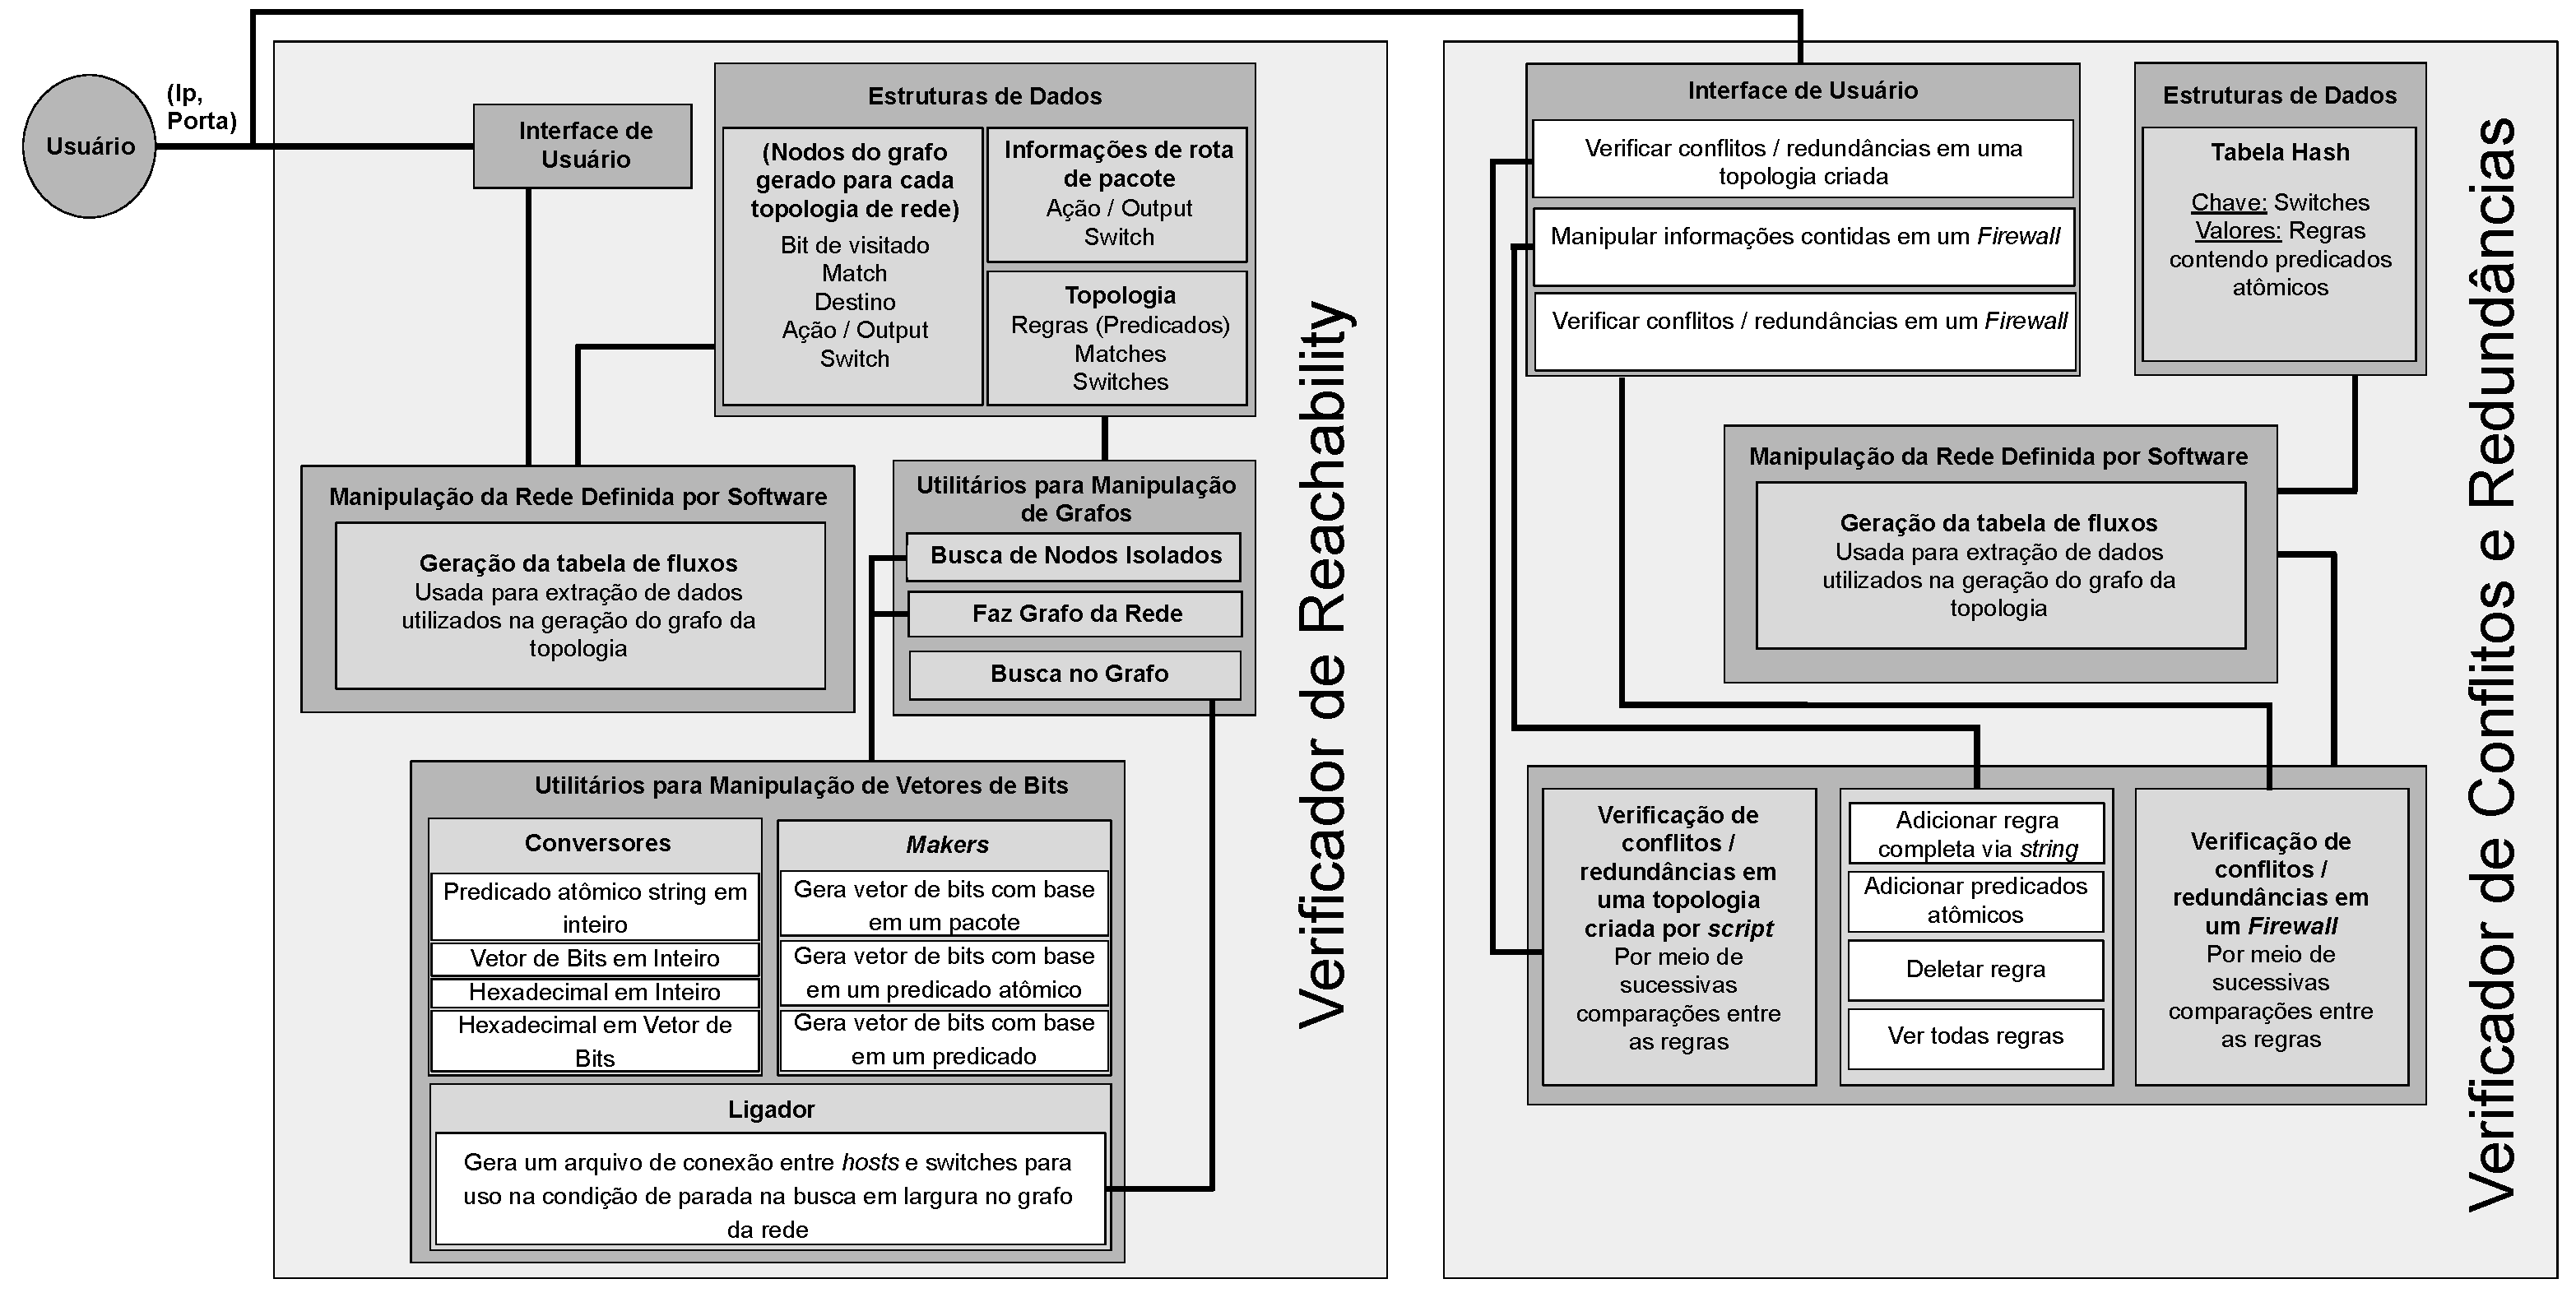
\includegraphics[width=\columnwidth, keepaspectratio]{Resources/ArquiteturaPlacidus.pdf}
     }
     \caption{Arquitetura proposta para a Plataforma Placidus. Fonte: obtido pelo autor, 2019.}
     \label{fig:ArquiteturaPlacidus}
 \end{figure}

\subsection{Módulo de Verificação de Conflitos e Redundâncias} 
Nesse módulo é feita a verificação  das propriedades de conflitos e redundâncias de regras de encaminhamento de pacotes, utilizando o protocolo OpenFlow.
Como é possível observar na Figura \ref{fig:ArquiteturaPlacidus}, é possível: (i) adicionar uma regra utilizando uma \textit{string} de caracteres, (ii) adicionar predicados atômicos, (iii) deletar uma regra e (iv) ver todas regras contidas no controlador \textit{SDN}.
No caso desse dispositivo, as ações referentes aos predicados podem ser "permitir" e "não permitir".

A ação de permitir é representada pelo número 1. Já a ação de não permitir a passagem de um pacote é representada pelo número 0 na tabela de fluxos do controlador \textit{floodlight}, o qual é utilizado pelo \textit{framework}.
A Figura \ref{fig:infosFloodlight} apresenta a organização da tabela de fluxos no controlador para um dispositivo de \textit{firewall}.
Além de verificação de propriedades e manipulação de \textit{firewalls}, é também possível, no Placidus, a verificação dessas em uma rede definida por software, a qual é montada com o auxílio de \textit{scripts} feitos na linguagem de programação Python\footnote{https://www.python.org}.
Essa verificação de propriedades é baseada em sucessivas comparações, duas a duas, dos dados de reconhecimento de pacotes (\textit{matches}) de cada regra.

\textbf{Comparações entre regras:} 
\begin{itemize}
    \item São feitas comparando de maneira exaustiva os dados de reconhecimento de pacotes (\textit{matches}) das regras.
    \item Cada regra é modelada como um predicado, o qual contém inúmeros predicados atômicos.
    \item Os predicados atômicos simbolizam as informações específicas de uma regra. Essas regras podem ser (i) IP de origem, (ii) IP de destino, (iii) prioridade, entre outras.
    \item São modeladas utilizando duplas sucessivas de regras, onde os índices dessas são dados por \textit{"cont1"} e \textit{"cont2"}, assim como mostrado na Figura \ref{fig:compsIterConfRedund}.
    \item As comparações entre os \textit{matches} das regras são feitas de maneira exaustiva, utilizando todos predicados atômicos contidos nos dados de reconhecimento de pacotes de cada regra.
    \item Por meio de inúmeras iterações, variando com o número de regras contidas na rede, são feitas verificações de igualdade de informações dos predicados atômicos entre as duplas de regras que estão sendo comparadas. Caso todos predicados atômicos da dupla sejam idênticos, é detectado conflito ou redundância entre regras.
\end{itemize}

A cada iteração, a primeira regra comparada é removida, e as comparações seguem acontecendo normalmente. 
Uma ilustração que apresenta o número de comparações dentro do laço de iterações pode ser vista na Figura \ref{fig:compsIterConfRedund}, onde as regras comparadas formam uma espécie de triângulo de comparações.
Essa remoção de uma regra a cada iteração acarreta em uma redução de 50\% no número de comparações em relação à ferramenta de verificação em \textit{firewalls} \textit{Formal Verification of Firewall Policies} \cite{Liu:2009}, que utiliza a comparação de todas regras entre si.

Na atual implementação do Placidus para verificação de conflitos, apenas \textit{matches} exatamente iguais são identificados. Contudo, está previsto o estudo para a implementação da verificação de regras que não possuem um \textit{match} idêntico, mas que conflitam por englobamento.
Além disso, mesmo que o OpenFlow faça desambiguação de regras através de regras de prioridade, o problema de espaço adicional ainda ocorre, uma vez que os switches possuem espaço limitado para alocação de regras.
Com muitas regras definidas, as não redundantes perdem espaço. Ademais, regras redundantes podem ser inseridas com a mesma regra de prioridade, o que acarreta no mesmo problema discutido anteriormente.

% Ilustração para a quantidade de comparações por iteração no módulo de conflitos e redundâncias
\begin{figure}[h!]
\centering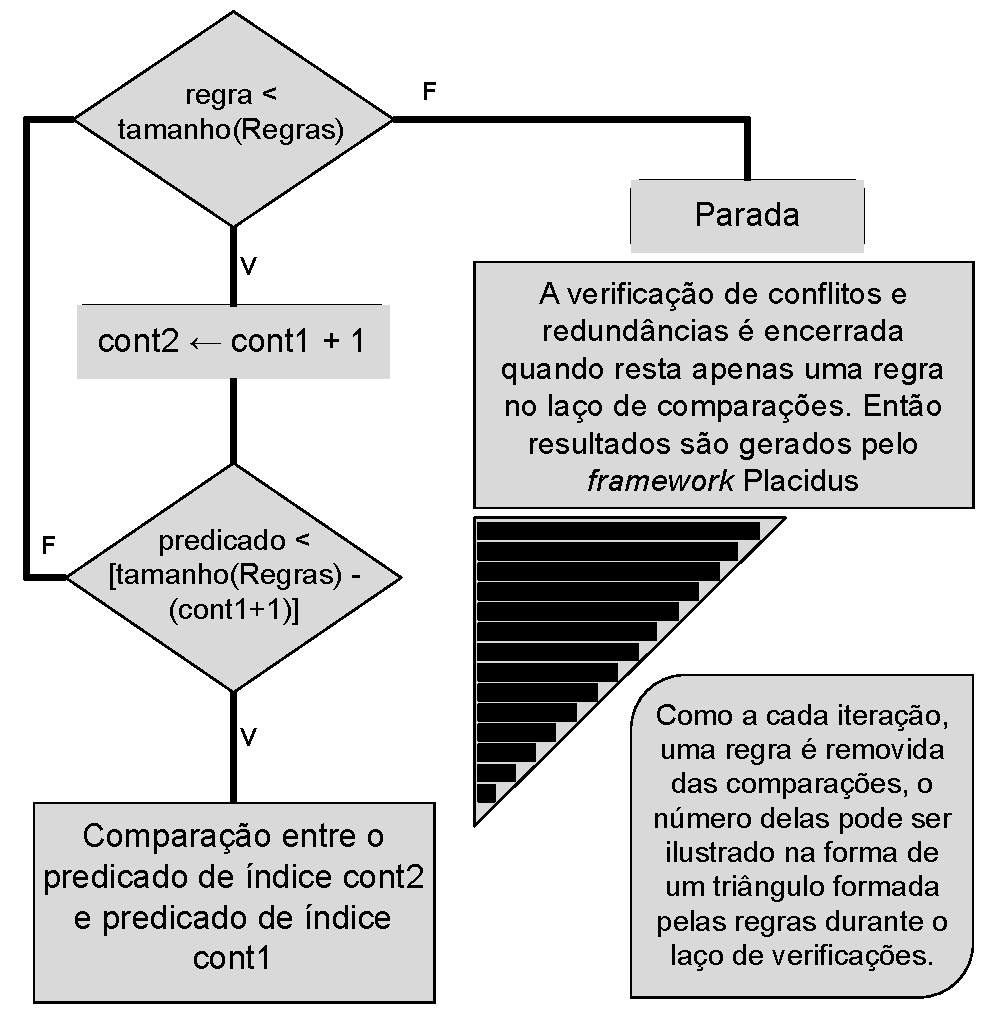
\includegraphics[width=.6\columnwidth]{Resources/CompsPorIteracaoConfRedund.pdf}
\caption{Comparações por Iteração no Módulo de Verificação de Conflitos e Redundâncias do Placidus. Fonte: obtido pelo autor, 2019.}
\label{fig:compsIterConfRedund}
\end{figure}

Após a verificação completa dos fluxos da rede, três arquivos são gerados: (i) com regras conflitantes, (ii) com regras redundantes e (iii) com todas as regras contidas na topologia de rede.
Cada linha desse arquivo é representada na forma de um produtório de informações de uma regra, que são os predicados atômicos, implicando na ação ou saída da mesma, conforme pode ser visto na Equação \ref{eq:formatoLinhasArq}.

% Equação para centralizar
\begin{equation}
\label{eq:formatoLinhasArq}
\prod_{i = 0}^{n\char`_infos} infoRegra_{i} \rightarrow Output 
\end{equation}

% Floodlight com Firewalls
\begin{figure}[h!]
\centering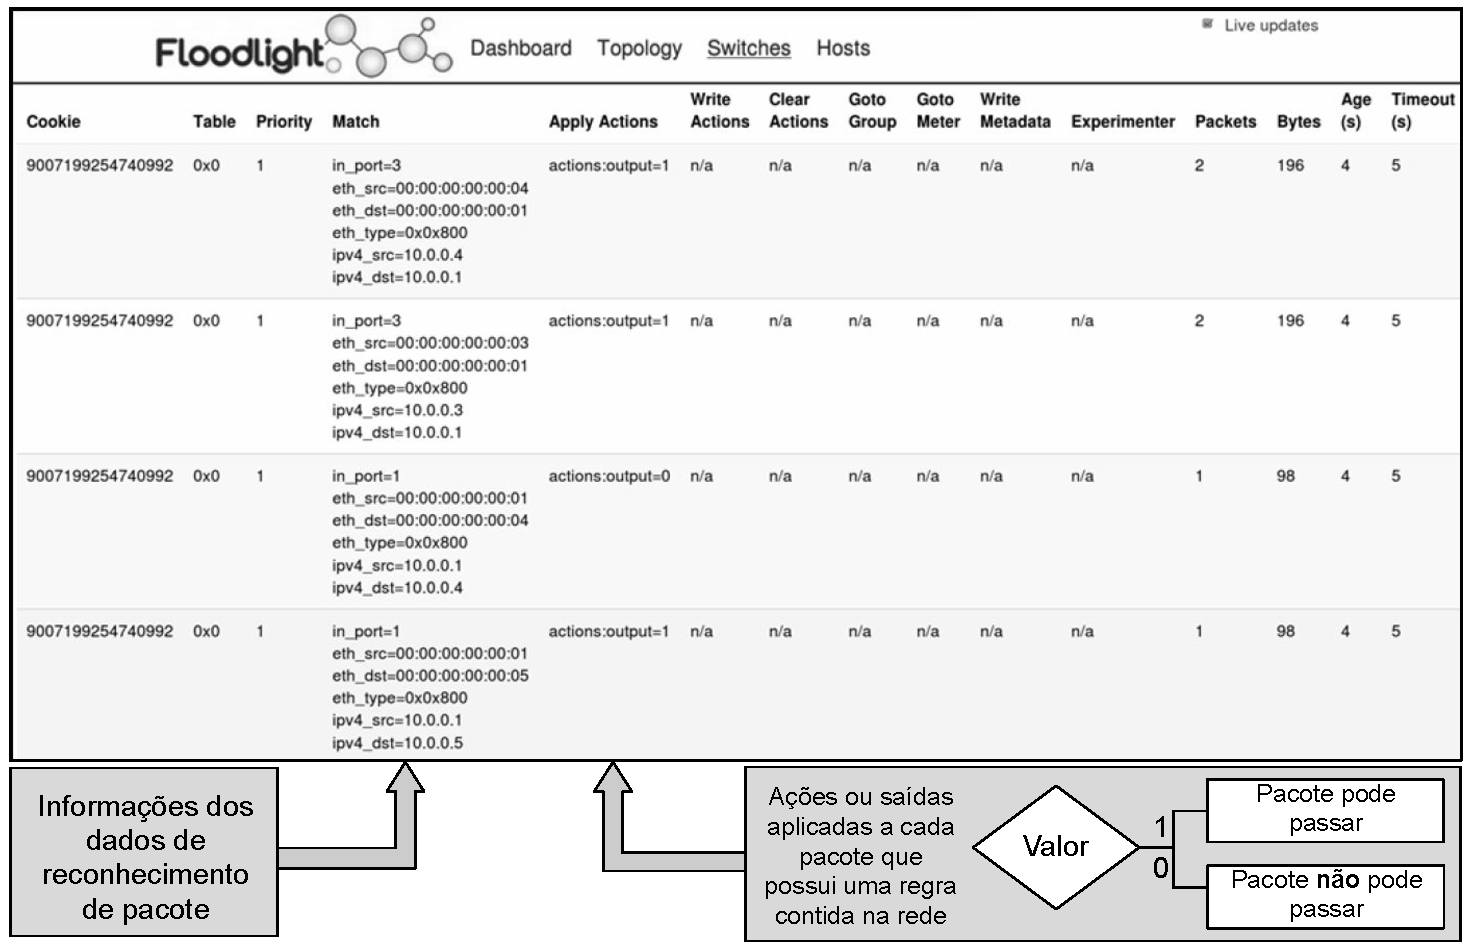
\includegraphics[width=\columnwidth]{Resources/InfosFloodlight.pdf}
\caption{Informações de um \textit{firewall} em uma tabela de fluxos do controlador Floodlight. Fonte: obtido pelo autor, 2019.}
\label{fig:infosFloodlight}
\end{figure}

\subsection{Módulo de Verificação de \textit{Reachability}} 
Nesse módulo é apresentado o bloco de verificação da propriedade de \textit{reachability} utilizando o protocolo OpenFlow.
Essa propriedade é verificada a partir do momento em que um pacote que sai de uma origem, e consegue chegar no destino especificado em seus dados de reconhecimento (\textit{match})  \cite{1498492}.
Diversos métodos foram criados, de modo a distribuir funcionalidades dentro do \textit{framework} e assegurar a facilidade na extensão do mesmo para verificação de outras propriedades em \textit{SDN}.
A primeira etapa do processo de verificação é a conversão das células da tabela de fluxos, gerada na etapa de coleta de dados. Todas células, as quais estão no formato de strings hexadecimais, são convertidas em vetores de \textit{bits}, utilizando a classe BitVector\footnote{https://pypi.python.org/pypi/BitVector/3.4.4}, juntamente a métodos específicos desenvolvidos para o \textit{framework} Placidus. 

Após ter a tabela com vetores de \textit{bits} que representam a rede, a mesma é utilizada para a montagem de um grafo de fluxos. Cada nodo desse grafo possui as seguintes informações: (i) \textit{match}, (ii) destino, (iii) ação ou saída, (iv) switch e (v) um \textit{bit} de visitado, o qual é utilizado na busca em largura no grafo da topologia. 
A verificação de \textit{reachability}, dado um pacote de entrada, consiste na busca em largura desse pacote no grafo montado.
Cada pacote contem duas informações: (i) \textit{Match} e (ii) destino. 
O \textit{match} é utilizado para achar o nodo em que inicia a busca, e o destino é utilizado como informação de parada. 
A propriedade de \textit{reachability} está correta, ao final da busca, se: (i) O destino do pacote for igual ao da última regra, (ii) o destino da regra pertencer ao switch que contém a mesma e (iii) o \textit{bit} de visitado do último nodo estiver ligado.

\subsection{Novos Módulos de Verificação, Integração com Banco de Dados e Infraestrutura}
Novos módulos de verificação formal no contexto de \textit{SDN} serão adicionados.
Um desses módulos, é o de checagem de \textit{black holes} dentro de uma topologia.
Um \textit{black hole}, no contexto de redes de computadores, é um lugar onde pacotes são destruídos ou descartados sem ter informação dada ao dispositivo que os enviou.
Ademais, ocorre também quando um pacote é perdido durante o envio, e nenhuma informação é dada ao dispositivo que o estava esperando.
\textit{Black holes} podem ocorrer por diversas circunstâncias.
Uma delas, por exemplo, é quando um roteador não alcançável por estar offline \cite{7396103}.
Outro módulo que será acoplado ao framework é o de verificação de \textit{slice isolation} dentro da rede. A propriedade de \textit{slice isolation} é um requirimento importante que permite garantir o conceito de núcleo da rede se particionando sobre a coexistência simultânea de múltiplos pedaços. Esses pedaços compartilham da mesma infraestrutura.
Essa propriedade é alcançada impondo que o desempenho de cada pedaço não deve impactar no dos outros \cite{8104638}.

Além disso, a plataforma contará com integração a um banco de dados não relacional, onde as chaves serão os identificadores de cada fluxo na rede.
Por fim, a plataforma completa será instalada em um servidor na nuvem, em uma máquina virtual da Microsoft Azure\footnote{https://azure.microsoft.com}, tendo seu \textit{deploy} automatizado.
Além disso, alguns métodos dos módulos poderão ser acessados via \textit{API (Application programming interface)}, podendo ser acessado de qualquer local, com os devidos cuidados com segurança da informação.

\subsection{Plano de Avaliação da Solução Proposta}
Para execução da solução proposta será usado o emulador de rede Mininet.
Além disso, o controlador \textit{SDN} que será utilizado é Floodlight OpenFlow.
As topologias serão criadas via scripts Python com o uso do pacote \textit{mininet}\footnote{http://mininet.org/download} e dos seguintes sub-módulos: (i) \textit{net}, (ii) \textit{topo}, (iii) \textit{log} e (iv) \textit{node}.

Os scripts farão a criação de switches openflow e de inúmeros \textit{hosts}\footnote{Dispositivo que é interligado com outra máquina através de conexão de Internet.} em diferentes topologias de redes.
O número de dispositivos influenciará na quantidade de fluxos gerados na rede.
A avaliação da solução se baseará principalmente em métricas de tempo e complexidade algorítmica, onde essas serão utilizadas para comparação com outros trabalhos da mesma área que o framework proposto.

\section{Cronograma de Atividades}
As atividades a serem realizadas na segunda parte do Trabalho de Graduação são as seguintes:

A. Aprimoramento do embasamento teórico: estudo mais aprofundado de técnicas atuais de verificação formal e suas abordagens para problemas como \textit{reachability}, \textit{slice isolation} e \textit{black hole} no contexto de redes definidas por software.

B. Implementação da solução: Desenvolvimento do framework Placidus para verificação das propriedades formais definidas, além da integração por meio de arquivos com o controlador Floodlight, conexão com um banco de dados para registro de eventos e infraestrutura na nuvem para o framework.

C. Criação dos cenários de teste: montagem das topologias de rede que serão utilizadas nos testes de verificação com o Placidus.

D. Análise dos resultados: consolidação dos resultados obtidos com a plataforma desenvolvida. Relacionar com o resultado de outros trabalhos da área no qual está inserida.

E. Redação da monografia: processo de formalização dos resultados obtidos, reunindo a conceituação teórica, os dados obtidos com os testes, comparativos e resultados alcançados com a solução desenvolvida.

F. Entrega e apresentação do trabalho: Revisar e entregar a monografia finalizada, além de apresentar o trabalho.

A Tabela \ref{table:cronograma} apresenta um cronograma para as atividades planejadas.

\begin{table}[h!]
\centering
\scalebox{0.7} {

\begin{tabular}{| c | c | c | c | c | c | c | c |} 
 \hline
       & Janeiro & Fevereiro & Março & Abril & Maio & Junho & Julho \\ [0.5ex] 
 \hline
 A. & \cellcolor{black} &   \cellcolor{black}  & & & & & \\
 \hline
 B. & \cellcolor{black}  & \cellcolor{black} & \cellcolor{black} & \cellcolor{black}  & \cellcolor{black} & & \\
 \hline
 C. &   &  &  & \cellcolor{black} & \cellcolor{black} & & \\
 \hline
 D. &   &   &  &  & \cellcolor{black} & \cellcolor{black} & \\
 \hline
 E. &  & &  \cellcolor{black}&  \cellcolor{black} &  \cellcolor{black} & \cellcolor{black} & \\ 
 \hline
 F. & & & & & & \cellcolor{black} &  \cellcolor{black} \\
 \hline 
\end{tabular}
}
\caption{Cronograma de atividades. Fonte: obtido pelo autor, 2019.}
\label{table:cronograma}
\end{table}

\bibliographystyle{sbc}
\bibliography{sbc-template}

\end{document}
